\chapter{ファイルの扱い方 --- Raw URL・画像・LFS}

\section{この章で学ぶこと}

GitHubは単なる「コードの保管庫」ではありません。リポジトリの中にあるファイルは、それぞれ固有のURLを持ち、特定の行を指し示したり、過去のある時点のスナップショットを永久に参照したりできます。さらに、画像や大容量ファイルの管理、別のリポジトリを取り込むサブモジュールなど、ファイルにまつわるさまざまな仕組みが用意されています。

この章では以下のことを学びます。

\begin{itemize}
  \item GitHub上のファイルURLの構造と、blob・tree・raw・blame・commitsの違い
  \item 特定の行へのリンクと、パーマリンク（永続リンク）の作り方
  \item Raw URLを使った生データの取得と、プログラムからの読み込み
  \item 画像をリポジトリに保存・表示する方法
  \item Git LFS（Large File Storage）で大容量ファイルを効率的に管理する方法
  \item サブモジュールでリポジトリの中に別のリポジトリを含める方法
  \item GitHub上でのファイル操作と便利なキーボードショートカット
\end{itemize}

\section{GitHub上のファイルURL構造 --- blob/tree/raw/blame/commitsの違いを詳しく}

GitHub上でファイルやフォルダを閲覧するとき、ブラウザのアドレスバーに表示されるURLには一定の規則があります。この規則を理解しておくと、他の人にファイルの場所を伝えたり、自動化スクリプトからファイルを取得したりする際に非常に役立ちます。

GitHubのファイルURLは、以下の構造になっています。

\begin{lstlisting}[language={}]
https://github.com/{owner}/{repo}/{表示モード}/{ブランチまたはコミット}/{ファイルパス}
\end{lstlisting}

ここで「表示モード」にあたる部分が、ファイルをどのような形で見るかを決定します。主な表示モードは5つあります。

\begin{table}[h]
\centering
\begin{tabular}{lll}
\hline
表示モード & 意味 & URLの例 \\
\hline
\cmd{blob} & ファイルの中身をシンタックスハイライト付きで表示 & \cmd{/blob/main/src/app.py} \\
\cmd{tree} & ディレクトリの中身（ファイル一覧）を表示 & \cmd{/tree/main/src/} \\
\cmd{raw} & ファイルの生データをそのまま返す（HTMLの装飾なし） & \cmd{/raw/main/data.csv} \\
\cmd{blame} & ファイルの各行を「誰がいつ変更したか」と共に表示 & \cmd{/blame/main/app.py} \\
\cmd{commits} & そのファイルに関するコミット履歴だけを表示 & \cmd{/commits/main/app.py} \\
\hline
\end{tabular}
\end{table}

\begin{figure}[htbp]
\centering
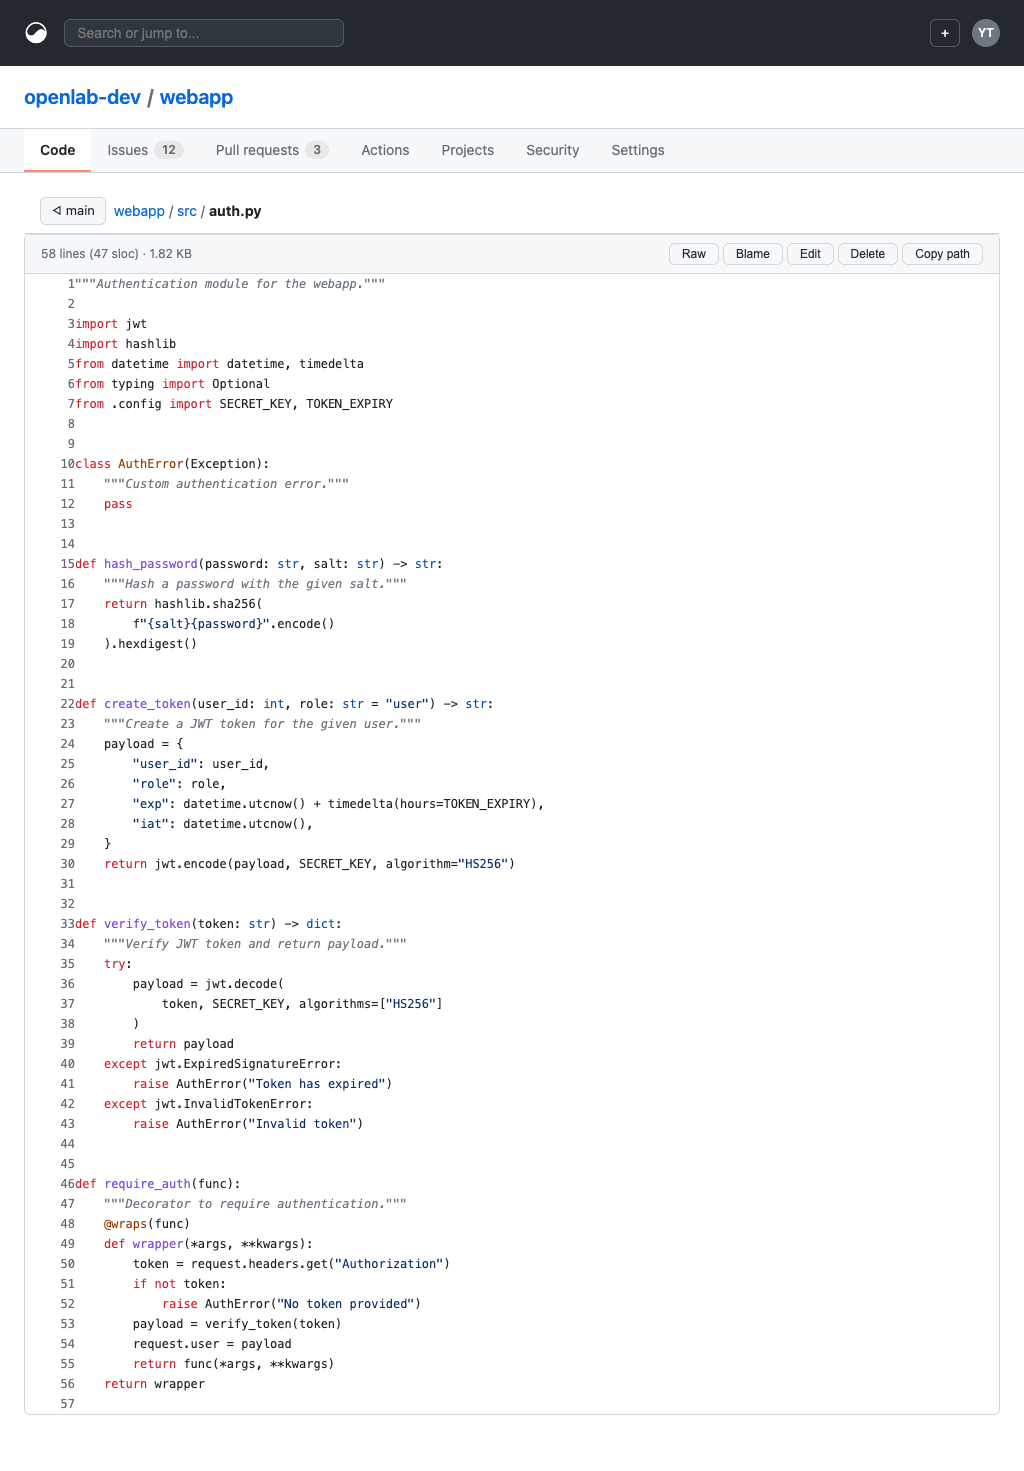
\includegraphics[width=0.95\textwidth]{images/file-blob.png}
\caption{blob表示とtree表示の比較}
\end{figure}

\textbf{blob} は最もよく使う表示モードです。リポジトリのファイル一覧からファイル名をクリックしたとき、自動的にこのモードで開かれます。コードにはシンタックスハイライトが適用され、行番号も表示されるため、読みやすい形で内容を確認できます。

\textbf{tree} はディレクトリを表示するモードです。リポジトリのトップページや、フォルダ名をクリックしたときに使われます。blob がファイル単体を表示するのに対し、tree はフォルダの中身の一覧を表示します。この名前はGitの内部データ構造に由来しています。Gitでは、ディレクトリを「tree オブジェクト」、ファイルを「blob オブジェクト」として管理しているのです。

\textbf{raw} はファイルの生データをそのまま返します。HTMLの装飾やヘッダー・フッターは一切なく、ファイルの中身だけが返されます。このモードは次のセクションで詳しく扱います。

\textbf{blame} は「git blame」コマンドのWeb版です。ファイルの各行について、「その行を最後に変更したのは誰か」「どのコミットで変更されたか」を表示します。バグの原因を追跡するときや、ある行がなぜそのように書かれているかを調べるときに重宝します。「blame（非難する）」という名前が少し物騒ですが、実際には「責任の所在を明らかにする」という意味合いで使われています。

\textbf{commits} はそのファイルに関係するコミットだけを時系列で表示します。リポジトリ全体のコミット履歴ではなく、特定のファイルがどのように変遷してきたかを追跡できるので、ファイルの変更履歴を調べるときに便利です。

\section{特定行へのリンクとパーマリンク}

\subsection{行番号リンク}

コードレビューやIssueの議論で「このファイルの42行目を見てほしい」と伝えたいことがあります。そんなとき、GitHub上のファイル表示画面で行番号をクリックすると、URLの末尾に \cmd{\#L42} が追加され、その行がハイライトされます。

\begin{lstlisting}[language={}]
# 42行目へのリンク
https://github.com/owner/repo/blob/main/src/app.py#L42

# 42行目から50行目までの範囲をハイライト
https://github.com/owner/repo/blob/main/src/app.py#L42-L50
\end{lstlisting}

範囲指定は、最初の行番号をクリックした後、Shiftキーを押しながら最後の行番号をクリックすることで設定できます。このURLをコピーしてIssueやPRのコメントに貼り付ければ、他のメンバーに正確な場所を伝えることができます。

\begin{figure}[htbp]
\centering
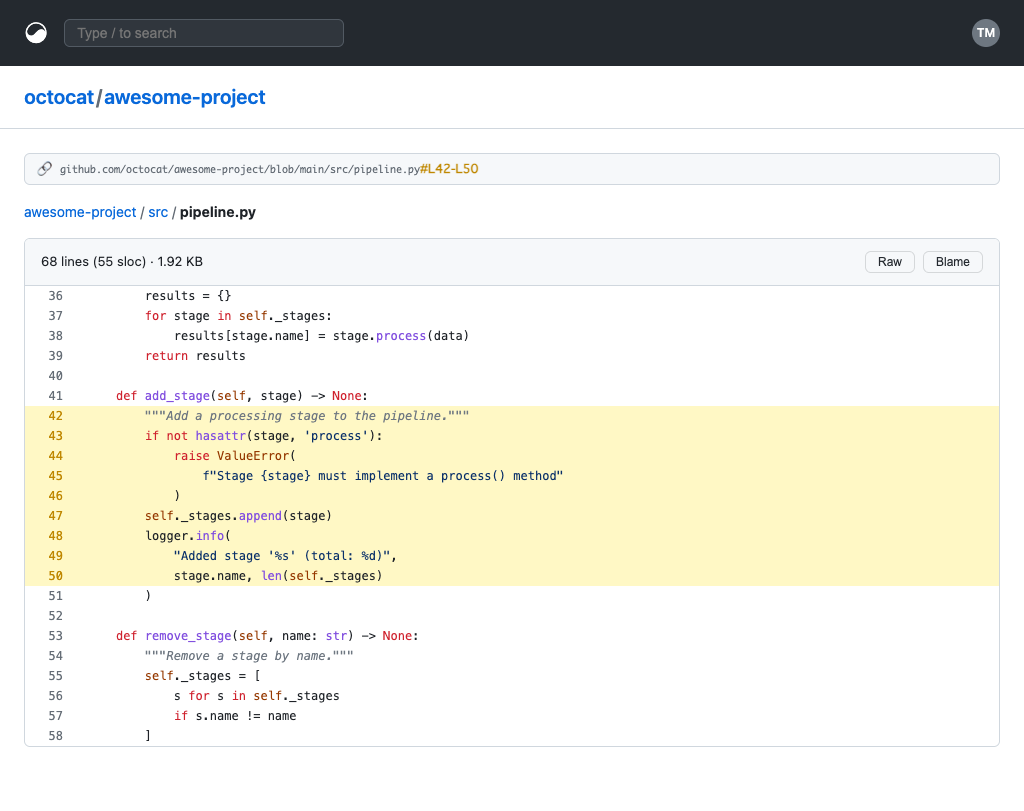
\includegraphics[width=0.95\textwidth]{images/line-highlight.png}
\caption{行番号をクリックしてハイライトされた状態}
\end{figure}

\subsection{パーマリンク --- なぜ永続リンクが重要なのか}

ここで一つ、重要な注意点があります。ブランチ名を含むURL（例えば \cmd{/blob/main/src/app.py\#L42}）は、ブランチの先端を指しています。つまり、誰かがそのファイルを編集してコミットすると、同じURLで表示される内容が変わってしまいます。42行目にあったコードが別の行に移動したり、まったく別の内容になっていたりする可能性があるのです。

これは、本の「最新版の42ページ」を参照するようなものです。改訂されれば42ページの内容は変わります。一方、「初版第3刷の42ページ」と言えば、いつ誰が参照しても同じ内容を指します。

Gitの世界では、この「初版第3刷」にあたるのがコミットハッシュです。コミットハッシュを含むURLは\textbf{パーマリンク（永続リンク）}と呼ばれ、未来永劫同じ内容を指し続けます。

\begin{lstlisting}[language={}]
# ブランチ指定（内容が変わりうる）
https://github.com/owner/repo/blob/main/src/app.py#L42

# コミットハッシュ指定（パーマリンク --- 永久に同じ内容）
https://github.com/owner/repo/blob/a1b2c3d4e5f6/src/app.py#L42
\end{lstlisting}

パーマリンクを手動で作るのは面倒ですが、GitHubには便利なショートカットがあります。ファイル表示画面で \textbf{\cmd{y}キー} を押すと、URLのブランチ名部分がその時点のコミットハッシュに自動的に置き換えられます。これだけでパーマリンクの完成です。

IssueやPRのコメント、ドキュメント、ブログ記事などでコードの特定箇所を参照するときは、必ずパーマリンクを使いましょう。ブランチ名を含むURLを貼ると、半年後にリンクをクリックした人が見る内容が、あなたが意図したものとまったく違っている可能性があります。

\section{Raw URL --- 生データの取得}

\subsection{Raw URLとは}

GitHubの通常のファイル表示（blob）は、HTMLページの中にコードが埋め込まれた形で表示されます。人間が読むには見やすいですが、プログラムからファイルの中身を取得したい場合には不便です。そこで登場するのが\textbf{Raw URL}です。

Raw URLはファイルの中身だけをそのまま返します。HTMLの装飾は一切ありません。CSVファイルならCSVデータそのもの、Pythonスクリプトならソースコードそのものが返されます。

Raw URLのドメインは \cmd{raw.githubusercontent.com} であり、通常のGitHubのURLとは異なります。

\begin{lstlisting}[language={}]
# 通常の表示URL（HTMLページとして表示される）
https://github.com/owner/repo/blob/main/data.csv

# Raw URL（ファイルの中身だけが返される）
https://raw.githubusercontent.com/owner/repo/main/data.csv
\end{lstlisting}

\subsection{curlでのダウンロード}

Raw URLを使えば、コマンドラインからファイルを直接ダウンロードできます。

\begin{lstlisting}[language=bash]
# ファイルをダウンロード
curl -O https://raw.githubusercontent.com/owner/repo/main/install.sh

# .gitignoreテンプレートをダウンロード
curl -o .gitignore https://raw.githubusercontent.com/github/gitignore/main/Python.gitignore

# シェルスクリプトを直接ダウンロードして実行（信頼できるソースに限る）
curl -fsSL https://raw.githubusercontent.com/owner/repo/main/setup.sh | bash
\end{lstlisting}

最後の例（ダウンロードして即実行）は便利ですが、信頼できるソースからのスクリプトに限って使うようにしてください。内容を確認せずに実行するのはセキュリティ上のリスクがあります。

\subsection{プログラムからの読み込み}

Raw URLはプログラムから直接データを読み込むのにも使えます。例えば、Pythonのpandasライブラリでは、URLを直接指定してCSVファイルを読み込めます。

\begin{lstlisting}[language=python]
import pandas as pd

# GitHubに置いたCSVデータを直接読み込む
url = "https://raw.githubusercontent.com/owner/repo/main/data.csv"
df = pd.read_csv(url)
print(df.head())
\end{lstlisting}

この方法は、データ分析のチュートリアルやサンプルコードでよく使われます。読者がデータをダウンロードする手間なく、コードをそのまま実行できるからです。ただし、大量のデータを繰り返し取得する場合は、ローカルにダウンロードしてから読み込む方が効率的です。

\section{画像の保存と表示}

GitHubのREADMEやドキュメントに画像を表示する方法は、主に2つあります。それぞれに利点と欠点があるので、用途に応じて使い分けましょう。

\subsection{方法1: リポジトリに画像ファイルを保存する}

最も正統派の方法は、リポジトリ内に画像ファイルを含めることです。プロジェクトの一部として画像をバージョン管理できるため、画像がなくなる心配がありません。

\begin{figure}[htbp]
\centering
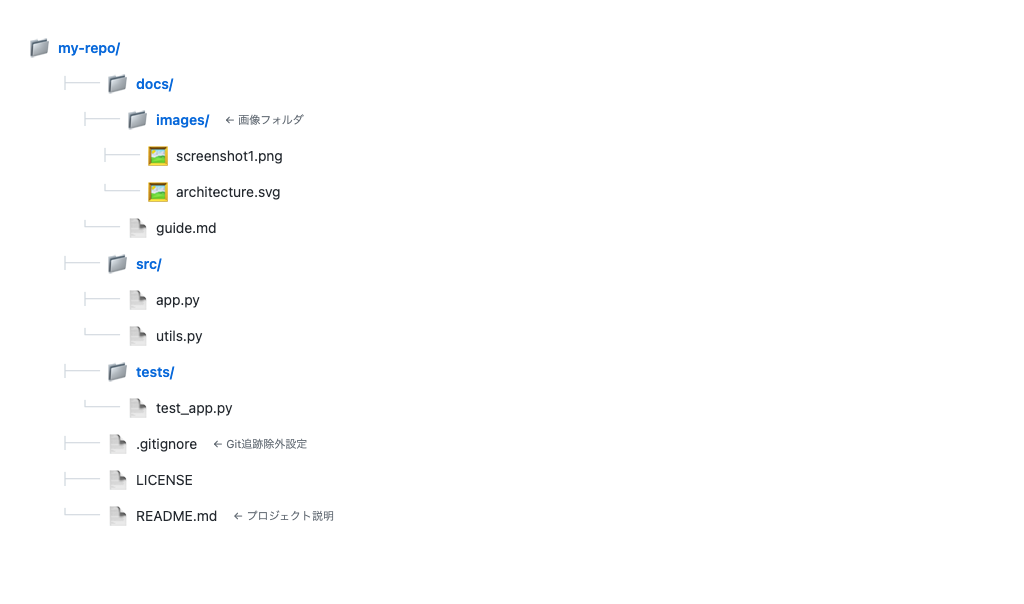
\includegraphics[width=0.9\textwidth]{images/diagram-file-tree.png}
\end{figure}

Markdownからは相対パスで参照します。

\begin{lstlisting}[language={}]
<!-- READMEから画像を参照する場合 -->
![スクリーンショット](docs/images/screenshot1.png)

<!-- docs/guide.md から同じフォルダの画像を参照する場合 -->
![アーキテクチャ図](images/architecture.svg)
\end{lstlisting}

SVG形式の画像はファイルサイズが小さく、拡大してもきれいに表示されるため、図やダイアグラムにはSVGがおすすめです。ただし、スクリーンショットのような写真的な画像にはPNGやJPEGが適しています。

この方法の注意点として、画像ファイルはバイナリデータであり、変更するたびにリポジトリのサイズが増えていくことがあります。大量の高解像度画像を含める場合は、後述するGit LFSの利用を検討してください。

\subsection{方法2: IssueにドラッグアンドドロップしてCDNを利用する}

もう一つの便利な方法は、GitHub自身のCDN（コンテンツ配信ネットワーク）を活用するやり方です。IssueやPull Requestのコメント欄に画像をドラッグアンドドロップすると、GitHubが自動的に画像をアップロードし、URLを生成してくれます。

\begin{figure}[htbp]
\centering
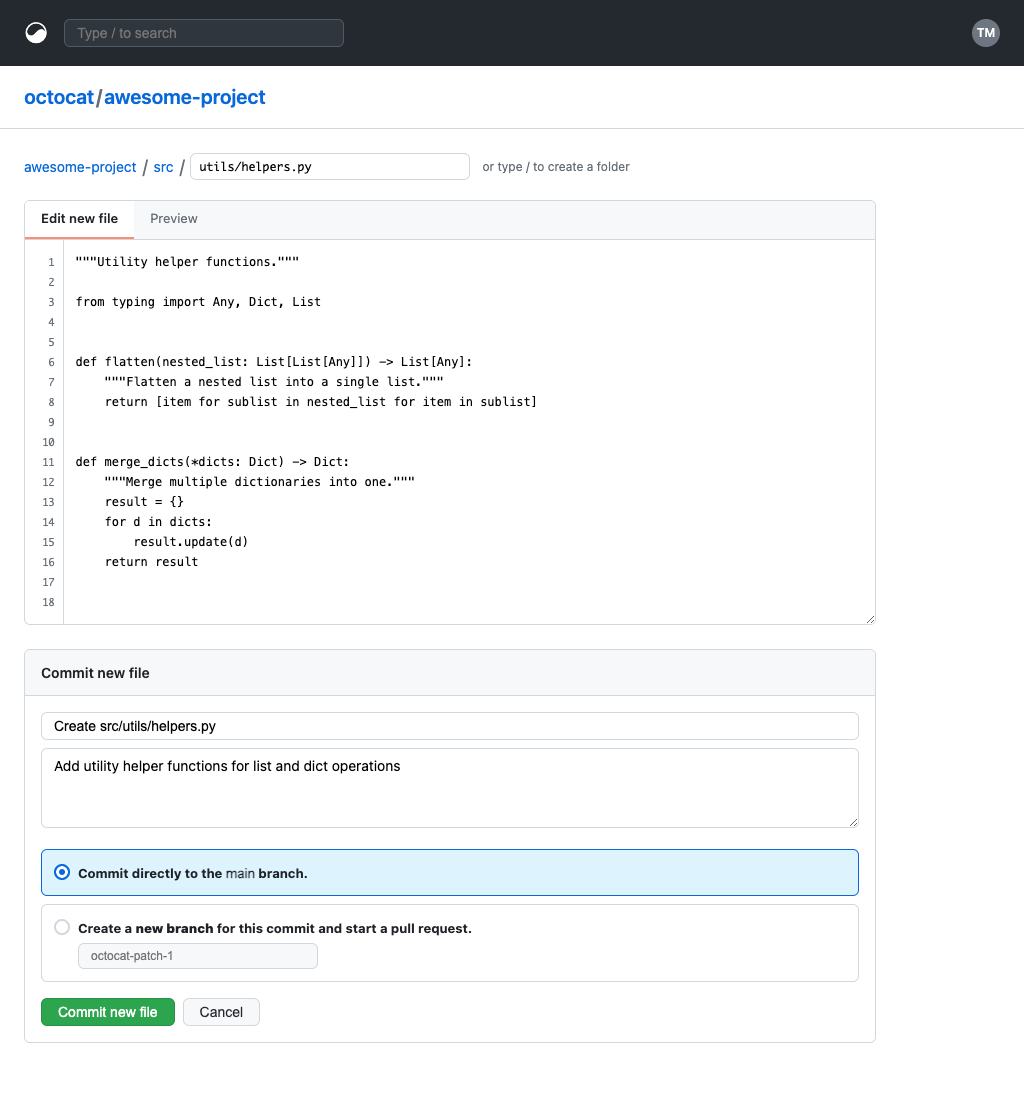
\includegraphics[width=0.95\textwidth]{images/file-create.png}
\caption{Issueのコメント欄に画像をドラッグアンドドロップする操作}
\end{figure}

生成されるURLは以下のような形式です。

\begin{lstlisting}[language={}]
https://github.com/user-attachments/assets/xxxxxxxx-xxxx-xxxx-xxxx-xxxxxxxxxxxx
\end{lstlisting}

このURLをREADMEや他のMarkdownファイルで使えば、リポジトリのサイズを増やさずに画像を表示できます。

\begin{lstlisting}[language={}]
![デモ画面](https://github.com/user-attachments/assets/xxxxxxxx-xxxx-xxxx-xxxx-xxxxxxxxxxxx)
\end{lstlisting}

ただし、この方法で生成されたURLがいつまで有効であるかはGitHubの裁量に依存します。長期的に重要な画像は、リポジトリに含める方法の方が確実です。

\subsection{HTMLタグでのサイズ指定}

Markdownの画像記法（\cmd{![alt](url)}）ではサイズを指定できません。画像が大きすぎる場合は、HTMLの \cmd{<img>} タグを使ってサイズを制御しましょう。

\begin{lstlisting}[language={}]
<!-- 幅を500ピクセルに指定（高さは自動調整） -->
<img src="docs/images/screenshot.png" width="500">

<!-- 幅と高さを両方指定 -->
<img src="docs/images/screenshot.png" width="400" height="300">

<!-- 中央寄せにする場合 -->
<p align="center">
  <img src="docs/images/logo.png" width="200">
</p>
\end{lstlisting}

GitHubのMarkdownレンダラーはHTMLタグの一部をサポートしています。\cmd{<img>} タグは問題なく使えるので、サイズの調整が必要な場合は積極的に活用しましょう。

\section{Git LFS --- 大容量ファイルの管理}

\subsection{なぜ大きなファイルが問題になるのか}

Gitは本来、テキストファイル（ソースコード）を管理するために設計されたツールです。テキストファイルであれば、差分（diff）を効率的に計算・保存できるため、ファイルが何千回変更されてもリポジトリのサイズはそれほど大きくなりません。

しかし、バイナリファイル（画像、動画、データセット、コンパイル済みバイナリなど）は事情が違います。Gitはバイナリファイルの差分を効率的に計算できないため、ファイルが変更されるたびにファイル全体のコピーが履歴に追加されます。例えば、100MBの画像ファイルを10回更新すると、リポジトリの履歴には約1GBのデータが蓄積されることになります。

リポジトリが肥大化すると、\cmd{git clone} に時間がかかり、ディスク容量を圧迫し、チーム全体の生産性が低下します。GitHubにはリポジトリサイズの推奨上限（5GB程度）もあります。

\subsection{LFSの仕組み --- ポインタファイル}

\textbf{Git LFS（Large File Storage）} はこの問題を解決するための拡張機能です。仕組みはシンプルです。大きなファイルの実体をリポジトリの外（LFS専用のストレージサーバー）に保管し、リポジトリには「ポインタ」だけを保存します。

ポインタファイルは数百バイト程度の小さなテキストファイルで、以下のような内容です。

\begin{lstlisting}[language={}]
version https://git-lfs.github.com/spec/v1
oid sha256:4cac19622fc3ada9c0fdeadb33f88f367b541f38b89de0ee093e6d0e2e13df38
size 104857600
\end{lstlisting}

\cmd{git clone} するとポインタファイルだけがダウンロードされるため高速です。ファイルの実体は、実際に必要になったとき（チェックアウトやdiffの際）に自動的にLFSサーバーからダウンロードされます。

\subsection{セットアップ手順}

\begin{lstlisting}[language=bash]
# 1. Git LFSのインストール
brew install git-lfs      # macOS (Homebrew)
apt install git-lfs        # Ubuntu/Debian

# 2. Git LFSの初期化（ユーザーごとに一度だけ実行）
git lfs install

# 3. 追跡するファイルパターンを指定
git lfs track "*.psd"           # Photoshopファイル
git lfs track "*.zip"           # ZIPアーカイブ
git lfs track "*.mp4"           # 動画ファイル
git lfs track "data/*.csv"      # dataフォルダ内のCSV

# 4. 自動生成された .gitattributes を確認
cat .gitattributes
# *.psd filter=lfs diff=lfs merge=lfs -text
# *.zip filter=lfs diff=lfs merge=lfs -text

# 5. .gitattributes をコミット（これが重要！）
git add .gitattributes
git commit -m "Configure Git LFS tracking"
\end{lstlisting}

\cmd{.gitattributes} ファイルは他のチームメンバーと共有されるため、必ずコミットしてください。これにより、リポジトリをクローンした全員が同じLFS設定を使えるようになります。

設定後は、通常通り \cmd{git add}、\cmd{git commit}、\cmd{git push} するだけです。LFSが追跡対象に指定されたファイルは、自動的にLFSストレージにアップロードされます。

\begin{lstlisting}[language=bash]
git add large-dataset.zip
git commit -m "Add training dataset"
git push
\end{lstlisting}

\subsection{容量制限}

GitHub上のLFSストレージには容量制限があります。

\begin{table}[h]
\centering
\begin{tabular}{lll}
\hline
プラン & ストレージ & 帯域幅（月あたり） \\
\hline
Free & 1 GB & 1 GB \\
Pro & 1 GB & 1 GB \\
追加データパック & +50 GB ストレージ / +50 GB 帯域（\$5/月） & \\
\hline
\end{tabular}
\end{table}

無料プランでも1GBまでは使えますが、それ以上のデータを扱う場合はデータパックの購入が必要です。大規模なデータセットを扱う研究プロジェクトなどでは、別のストレージサービス（S3やGCSなど）を併用することも検討しましょう。

\section{サブモジュール --- リポジトリの中に別リポジトリを含める}

\subsection{サブモジュールとは}

開発を進めていると、「複数のプロジェクトで共通して使うライブラリ」を別リポジトリとして管理したい場面が出てきます。このとき、共通ライブラリのコードをコピーして各プロジェクトに含めると、更新の反映が面倒になります。かといって、パッケージマネージャー経由で配布するほど大げさなものでもない場合もあるでしょう。

\textbf{サブモジュール（submodule）} は、あるリポジトリの中に別のリポジトリを「入れ子」にする仕組みです。親リポジトリは、子リポジトリの特定のコミットへの参照を保持します。

\begin{figure}[htbp]
\centering
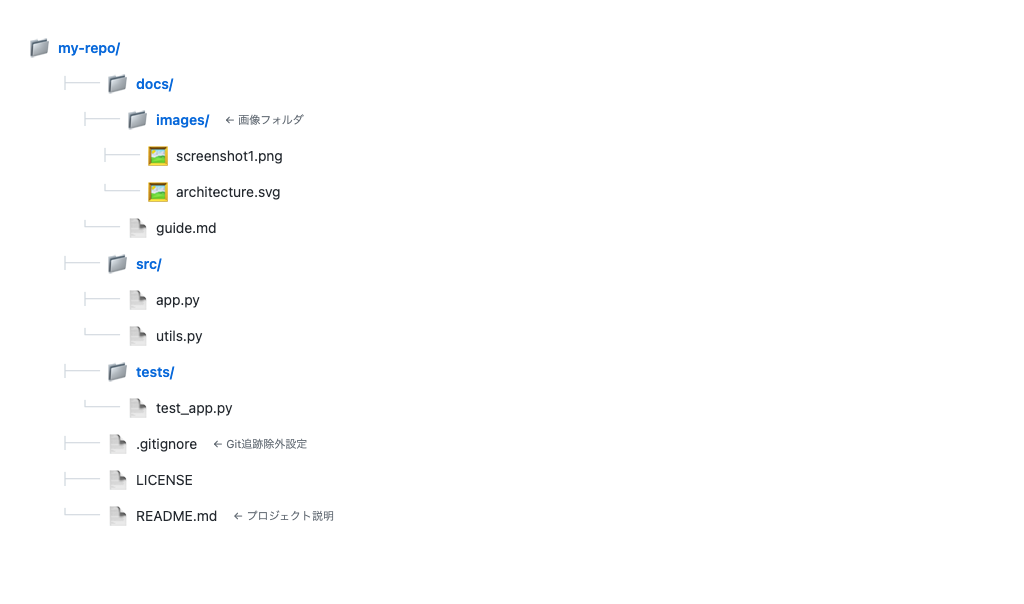
\includegraphics[width=0.9\textwidth]{images/diagram-file-tree.png}
\end{figure}

\subsection{サブモジュールの追加}

\begin{lstlisting}[language=bash]
# サブモジュールを追加（lib/shared-utils/ に配置）
git submodule add git@github.com:owner/shared-utils.git lib/shared-utils

# .gitmodules ファイルが自動的に作成される
cat .gitmodules
# [submodule "lib/shared-utils"]
#     path = lib/shared-utils
#     url = git@github.com:owner/shared-utils.git

# 設定をコミット
git add .gitmodules lib/shared-utils
git commit -m "Add shared-utils as submodule"
\end{lstlisting}

\subsection{サブモジュール付きリポジトリのクローン}

サブモジュールを含むリポジトリをクローンする際は、\cmd{--recursive} オプションを付ける必要があります。このオプションを忘れると、サブモジュールのディレクトリは空のままになります。

\begin{lstlisting}[language=bash]
# クローンと同時にサブモジュールも取得（推奨）
git clone --recursive git@github.com:owner/my-project.git

# すでにクローン済みの場合は、後からサブモジュールを取得
cd my-project
git submodule init
git submodule update
\end{lstlisting}

\subsection{サブモジュールの更新}

サブモジュールの元リポジトリに新しいコミットが追加された場合、親リポジトリ側で明示的に更新する必要があります。

\begin{lstlisting}[language=bash]
# サブモジュールを最新のコミットに更新
cd lib/shared-utils
git pull origin main
cd ../..

# 親リポジトリでサブモジュールの更新をコミット
git add lib/shared-utils
git commit -m "Update shared-utils submodule"

# または、一括で全サブモジュールを更新
git submodule update --remote --merge
\end{lstlisting}

サブモジュールは強力な仕組みですが、チームメンバーがサブモジュールの概念を理解していないと混乱の原因になることもあります。使用する際はREADMEにサブモジュールの存在と、\cmd{--recursive} でのクローンが必要である旨を記載しておくとよいでしょう。

\section{GitHub上でのファイル操作}

Gitコマンドやエディタを使わずに、GitHubのWeb画面上でもファイルの作成・編集ができます。ちょっとしたタイポの修正やドキュメントの更新には、Web上で直接編集する方が手軽です。

\subsection{ファイルの作成}

\begin{enumerate}
  \item リポジトリのページを開く
  \item 「\textbf{Add file}」ボタンをクリックし、「\textbf{Create new file}」を選択
  \item ファイル名の入力欄にパスを入力（スラッシュを含めるとフォルダが自動作成される）
  \item エディタにファイルの内容を入力
  \item 「\textbf{Commit changes}」をクリック
\end{enumerate}

\begin{figure}[htbp]
\centering
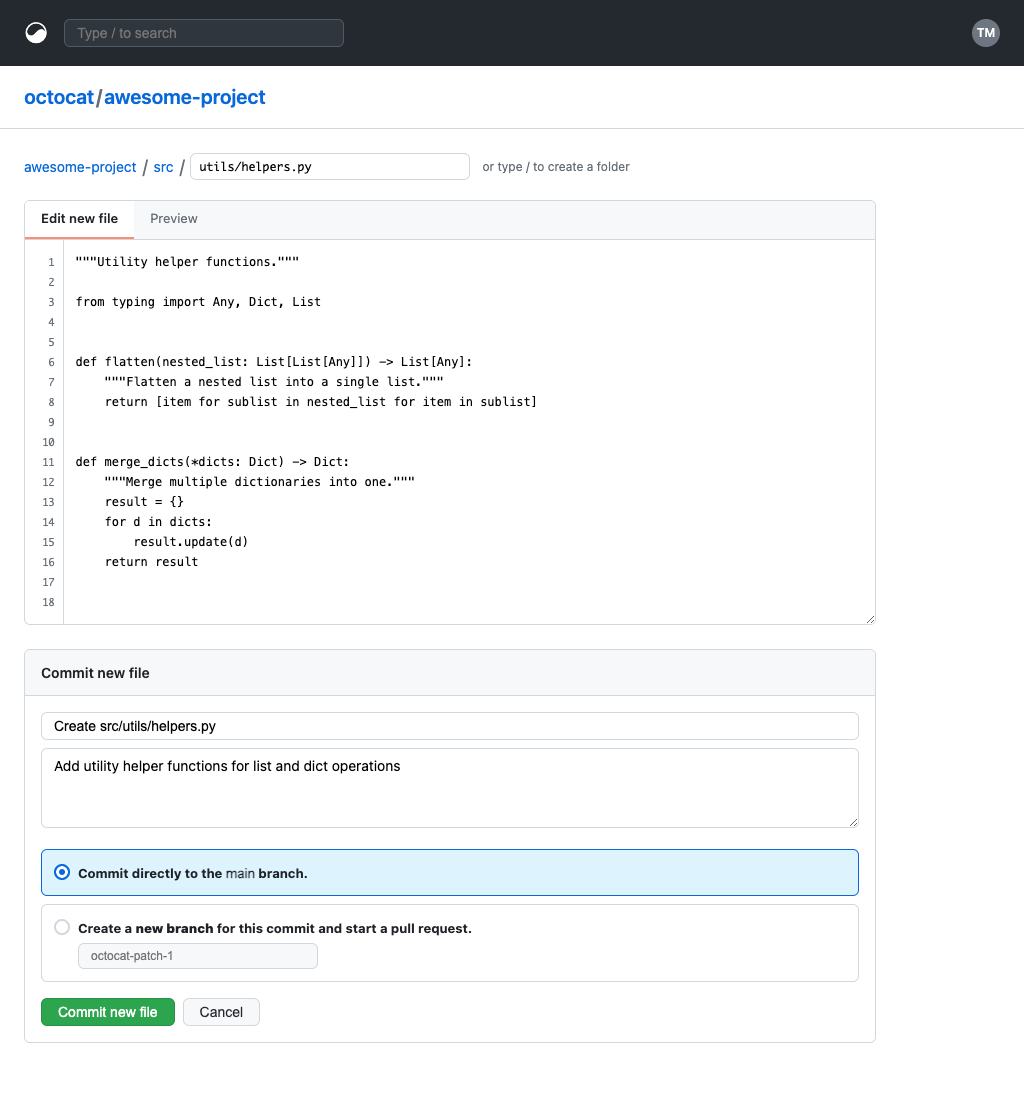
\includegraphics[width=0.95\textwidth]{images/file-create.png}
\caption{GitHub上でのファイル作成画面}
\end{figure}

例えば、ファイル名の入力欄に \cmd{docs/guide/getting-started.md} と入力すると、\cmd{docs/guide/} というフォルダ構造が自動的に作成され、その中に \cmd{getting-started.md} が作られます。

\subsection{ファイルの編集}

既存のファイルを表示した状態で、鉛筆アイコン（Edit）をクリックすると、その場で編集できます。編集後は通常のコミットと同様に、コミットメッセージを入力して保存します。直接mainブランチにコミットすることも、新しいブランチを作ってPull Requestを開くこともできます。

\subsection{キーボードショートカットによる検索}

GitHub上でファイルを探すとき、マウスでフォルダを一つずつ開いていくのは非効率です。以下のキーボードショートカットを覚えておくと、素早くファイルを見つけられます。

\begin{table}[h]
\centering
\begin{tabular}{ll}
\hline
キー & 機能 \\
\hline
\cmd{t} & ファイルファインダーを開く（ファイル名のファジー検索） \\
\cmd{s} または \cmd{/} & リポジトリ内の検索バーにフォーカス \\
\hline
\end{tabular}
\end{table}

\textbf{\cmd{t}キー}は特に便利です。リポジトリのどのページにいても \cmd{t} を押すと、ファイル名を部分一致で検索できるファインダーが開きます。例えば「conf」と入力すれば、\cmd{config.yml}、\cmd{.prettierrc.conf}、\cmd{settings/configuration.py} などが候補に表示されます。大規模なリポジトリでファイルを探すときに重宝するショートカットです。

\begin{figure}[htbp]
\centering
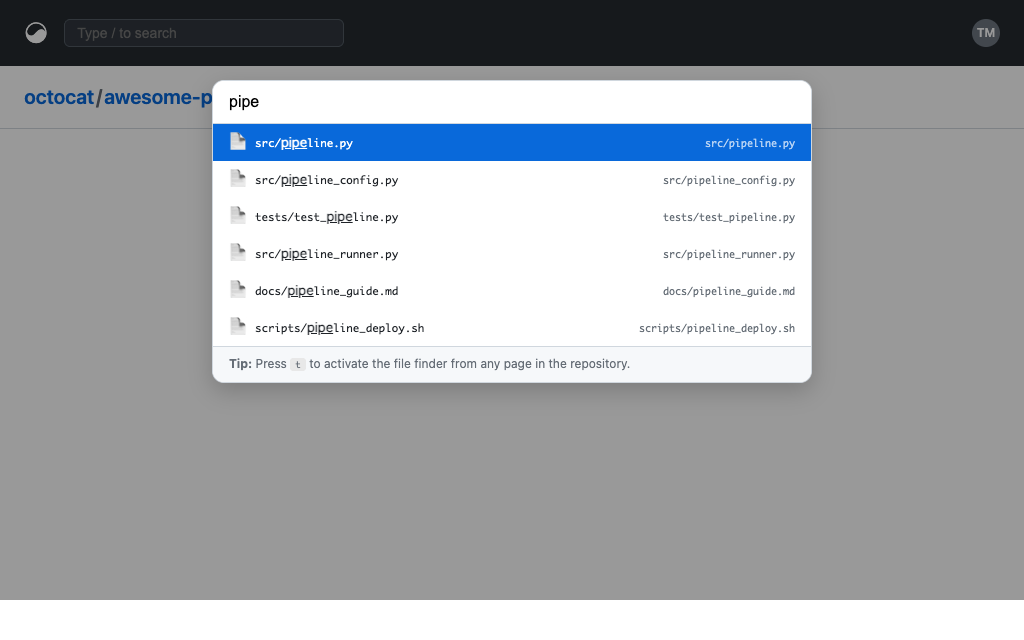
\includegraphics[width=0.95\textwidth]{images/file-finder.png}
\caption{tキーで開くファイルファインダー}
\end{figure}

\section{まとめ}

この章では、GitHub上でのファイルの扱い方を幅広く学びました。

\begin{itemize}
  \item \textbf{URL構造}: blob（ファイル表示）、tree（ディレクトリ表示）、raw（生データ）、blame（行ごとの変更者）、commits（ファイルの変更履歴）の5つの表示モードがある
  \item \textbf{行番号リンク}: \cmd{\#L42} や \cmd{\#L42-L50} で特定行を指し示せる
  \item \textbf{パーマリンク}: \cmd{y} キーでブランチ指定URLをコミットハッシュ指定に変換でき、内容が変わらない永続リンクを作れる
  \item \textbf{Raw URL}: \cmd{raw.githubusercontent.com} から生データを取得でき、curlやプログラムから直接読み込める
  \item \textbf{画像}: リポジトリに保存する方法とIssueにD\&DしてCDNを使う方法がある。HTMLの \cmd{<img>} タグでサイズ指定が可能
  \item \textbf{Git LFS}: 大容量のバイナリファイルはポインタだけをGitに保存し、実体は別サーバーに保管する仕組み
  \item \textbf{サブモジュール}: リポジトリの中に別リポジトリを入れ子にでき、\cmd{--recursive} オプションでクローンする
  \item \textbf{Web上のファイル操作}: ブラウザ上でファイルの作成・編集ができ、\cmd{t} キーでファイルを素早く検索できる
\end{itemize}
